% Preamble
\documentclass[paper=a4, fontsize=10pt]{scrartcl}
% Settings for the document
\setlength{\paperheight}{11in}
\setlength{\paperwidth}{8.5in}

% Packages to include
\usepackage{amsmath}
\usepackage{color}
\usepackage[left=0.75in, right=0.75in, top=0.75in, bottom=0.75in]{geometry}
\usepackage{graphicx}
\usepackage{mathptmx}
\usepackage{mathtools}

% Location for figures
\graphicspath{{./figures/}}

%%%%% MY COMMANDS %%%%%


% Maketitle Metadata
\title{
		\vspace{-1in} 	
		\usefont{OT1}{bch}{b}{n}
		\normalfont \large \textsc{ECE 189A - Eternal Flight} \\ [10pt]
		\rule{\linewidth}{2pt} \\ [0.4cm]
		\Huge Milestone 4 \\
		\LARGE Detailed Design Checklist \\
		\rule{\linewidth}{2pt}
}
\author{
		\normalfont 
		\large Richard Boone, Kyle Douglas, Sayali Kakade, \\
		\large Sang Min Oh, \& Aditya Wadaskar \\ [-3pt]		 			%\large \today
}
\date{}

% Begin document
\begin{document}
\maketitle

%%%%%%%%%%%% BEGIN DOCUMENT CONTENT %%%%%%%%%%%%
\vspace{-0.5in}%
\section{Intended Software Structure}
\subsection*{Parent Drone}
The parent drone has one on-board computer, a Raspberry Pi 3 B+, which will run Raspbian Lite (a headless Debian-based Linux distribution). The following table outlines the hardware-software interactions and the layout of the software with respect to each of the modules that will need to be programmed for interaction with the Raspberry Pi.\\%
\begin{table}[h!]
	\centering
	\begin{tabular}{|l|p{0.6\textwidth}|}
		\hline
		\textbf{Hardware Connections to Software} & \textbf{Purpose of Software}\\%
		\hline
		\hline
		USB1 $\rightarrow$ DJI N3 Flight Controller & UART connection: sends directional instructions to the parent drone to control its movement. We will explore the exact interfacing and API calls further.\\%
		\hline
		USB2 $\rightarrow$ Wifi Adapter & USB connection: acts as a fail-safe for the DGPS module. It allows remote access to the Raspberry Pi for other communications between the parent and child drones, if necessary.\\%
		\hline
		USB3 $\rightarrow$ ublox DGPS Module & USB connection: provides RTK positioning, with the parent drone acting as the moving baseline in relation to the child drone.\\%
		\hline
		GPIO Pin 2 $\rightarrow$ Linear Actuator & Applies a linear force to move batteries in and out of the battery-switching contraption on the child drone.\\%
		\hline
	\end{tabular}
\end{table}
\hfill\\%
The structure of the software on the Raspberry Pi 3 B+ will be as follows:\\%
\\%
\textbf{State 1: Deactivated -- The parent drone is not searching for the child drone}\\%
\begin{algorithm}[H]
	\While{parent drone not activated}{
		ignore child drone\;
	}
	transition to state 2\;
\end{algorithm}

\hfill\\%
\textbf{State 2: Activated -- The parent drone is actively searching for the child drone}\\%
\begin{algorithm}[H]
	\While{no communication with child drone}{
		establish communication over WIFI with child drone\;
	}
	retrieve GPS coordinate of child drone\;
	fly to \textit{N} feet below child drone and hover\;
    activate electromagnets in preparation for the child drone landing\;
	\While{child drone not latched to parent}{
		hover in place\;
	}
	transition to state 3\;
\end{algorithm}
\newpage\noindent
\textbf{State 3: Battery Switching -- The child drone is latched onto the parent drone}\\%
\begin{algorithm}[H]
	activate linear actuator\;
	insert new battery into child drone and push out stale battery\;
	signal child drone to power on and unlatch from parent drone\;
	\While{signal acknowledgment not received from child drone}{
		keep electromagnets activated\;
	}
	deactivate electromagnets\;
	\While{child is latched onto parent}{
		hover in place\;
	}
	transition back to state 1\;
\end{algorithm}

\subsection*{Child Drone}
The child drone will also have an on-board computer, a Raspberry Pi Zero W, which will also run Raspbian Lite. The child drone will have a PixRacer flight controller, which will be running the px4 flight control framework. The following table outlines the hardware-software interactions and the layout of the software for the child drone's on-board computer.
\begin{table}[h!]
	\centering
	\begin{tabular}{|p{0.35\textwidth}|p{0.6\textwidth}|}
		\hline
		\textbf{Hardware Connections to Software} & \textbf{Purpose of Software}\\%
		\hline
		\hline
		USB $\rightarrow$ Telemetry1 of PixRacer & Serial port connection: controls the movement of the child drone motors using directional commands.\\%
		\hline
		GPIO 4, 6 $\rightarrow$ Step-Down Converter & Steps-down the battery voltage from 14.7 V to 5 V for powering other peripherals.\\%
		\hline
		GPIO 8, 10 $\rightarrow$ OpenMV P4/P5 (TX/RX) & $\text{I}^2\text{C}$ connection: communicates the location in which the AprilTag (and thus, the parent drone) is detected.\\%
		\hline
		UART $\rightarrow$ ublox DGPS Module & Gets the current location of the parent drone with the child drone acting as the rover in the ublox RTK moving baseline model.\\%
		\hline
	\end{tabular}
\end{table}
\hfill\\%
The structure of the software on the Raspberry Pi Zero W will be as follows:
\hfill\\%
\textbf{State 1: Deactivated -- The parent drone is not searching for the child drone}\\%
\begin{algorithm}[H]
	\While{parent drone not activated}{
		remain stationary\;
	}
	transition to state 2\;
\end{algorithm}
\hfill\\%
\textbf{State 2: Activated -- The child drone is hovering and waiting for the parent drone}\\%
\begin{algorithm}[H]
	\While{AprilTag not detected}{
		hover in place\;
	}
	\While{child drone not latched to parent drone}{
		read AprilTag information from OpenMV\;
		provide directions to PixRacer to descend and land on parent drone\;
	}
	signal to the parent drone indicating successful latch\;
	transition to state 3\;
\end{algorithm}
\hfill\\%
\textbf{State 3: Battery Switching -- The child drone is latched onto the parent drone}\\%
\begin{algorithm}[H]
	\While{signal to unlatch not received from parent drone}{
		remain stationary on top of the parent drone\;
	}
	supply power to motors\;
	send acknowledgment of signal to parent drone\;
	rapidly take off from the parent drone\;
	transition back to state 2\;
\end{algorithm}	

\newpage
\section{Schematics}
\begin{figure}[h!]
	\centering
	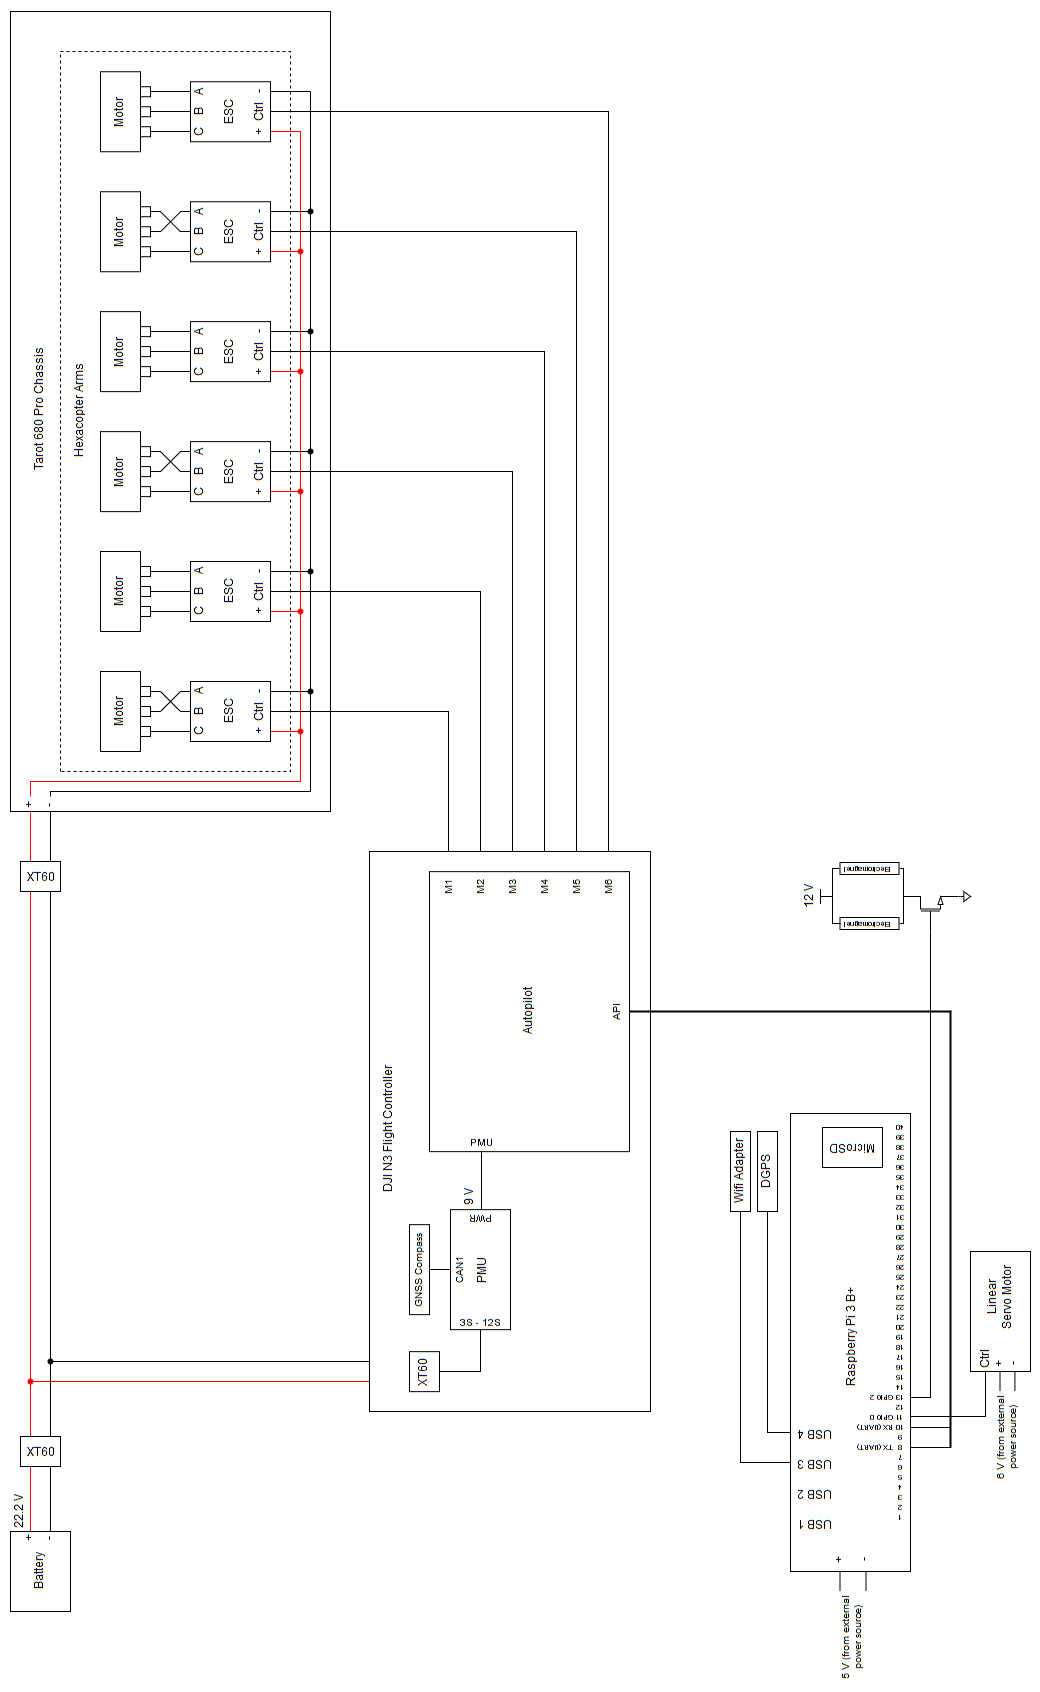
\includegraphics[width=0.87\textwidth]{parentedit}
	\caption{Parent Drone Schematic}
\end{figure}
\newpage
\begin{figure}[h!]
	\centering
	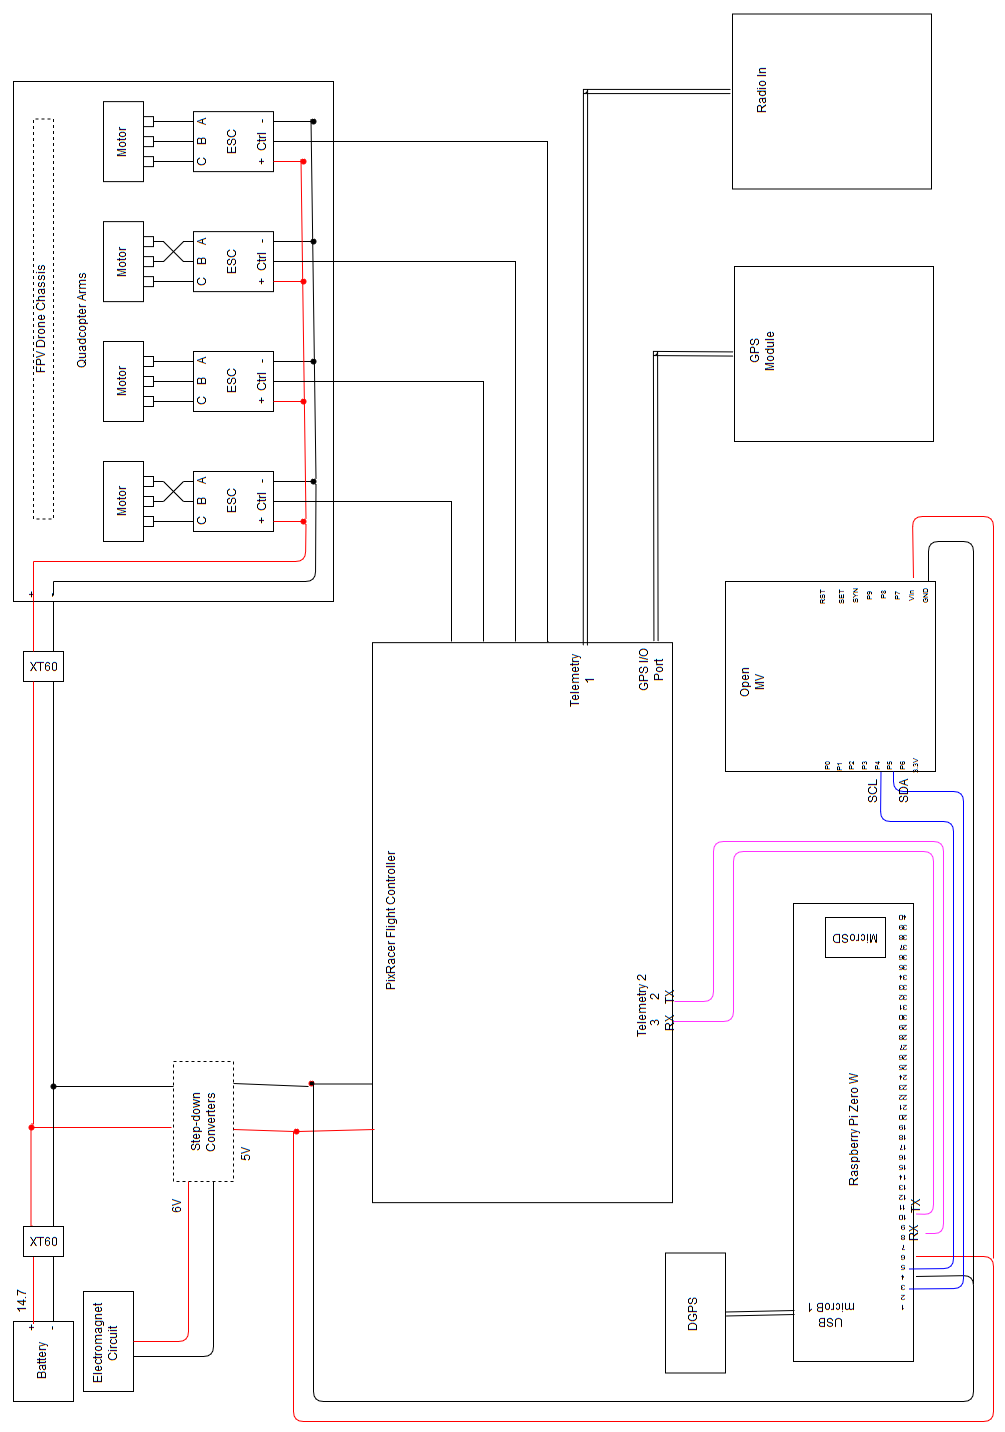
\includegraphics[width=0.95\textwidth]{childedit}
	\caption{Child Drone Schematic}
\end{figure}

%%%%%%%%%%%%% END DOCUMENT CONTENT %%%%%%%%%%%%%

%%%%%%%%%%%%%%% BEGIN REFERENCES %%%%%%%%%%%%%%%

%%%%%%%%%%%%%%%% END REFERENCES %%%%%%%%%%%%%%%%

% End document
\end{document}